

We explore the tool using the given example. \\

Let's answer the few questions asked at the end of this part.
\\

\smallskip
\begin{itemize}
    \item What do we observe when we check the inferred classes ?
\end{itemize}
\smallskip
Answer :    The inferred classes are the same as the asserted classes. This means that there are no additional logical consequences or inferences made by the reasoner beyond what has already been explicitly asserted in the ontology. This indicates that the ontology is consistent, and the asserted hierarchy or relationships between classes are correctly modeled according to the ontology's logical structure.

\begin{itemize}
    \item Some DL queries examples and results.
\end{itemize}

\begin{figure}[H]
    \centering
    \begin{minipage}[b]{0.25\textwidth}
        \centering
        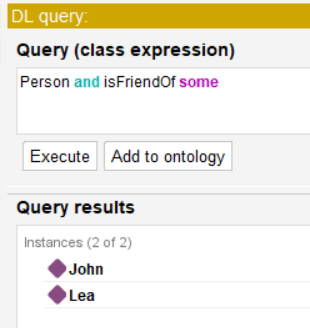
\includegraphics[width=\textwidth]{images/1.1 - tuto/DL query.png}
        \caption{DL query : Persons who have friends}
        \label{fig:image1}
    \end{minipage}
    \hfill
    \begin{minipage}[b]{0.25\textwidth}
        \centering
        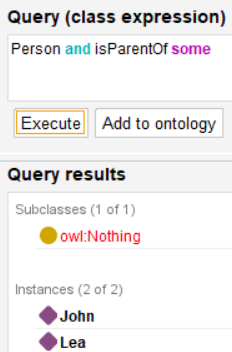
\includegraphics[width=\textwidth]{images/1.1 - tuto/q2.png}
        \caption{Persons who are Parents}
        \label{fig:image2}
    \end{minipage}
    \hfill
    \begin{minipage}[b]{0.25\textwidth}
        \centering
        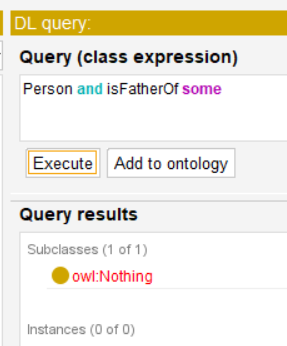
\includegraphics[width=\textwidth]{images/1.1 - tuto/q3.png}
        \caption{Persons who are Fathers : Issue there}
        \label{fig:image3}
    \end{minipage}
    
    \vspace{0.5cm} % Add vertical space between the rows
    
    \begin{minipage}[b]{0.4\textwidth}
        \centering
        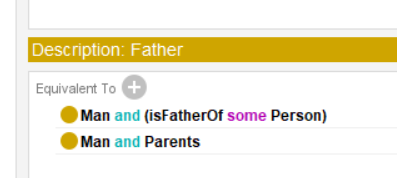
\includegraphics[width=\textwidth]{images/1.1 - tuto/q4 - adding an axiom to father .png}
        \caption{Adding two axiom to the Father Class}
        \label{fig:image4}
    \end{minipage}
    \hfill
    \begin{minipage}[b]{0.25\textwidth}
        \centering
        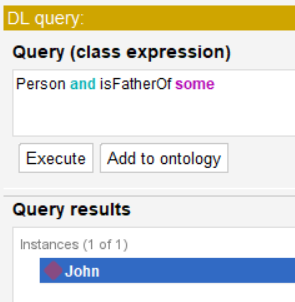
\includegraphics[width=\textwidth]{images/1.1 - tuto/q5 - now q3 works .png}
        \caption{This enabled the reasoner to infer that John is a Father}
        \label{fig:image5}
    \end{minipage}
    \caption{All Images Displayed in Two Rows with Harmonized Widths}
    \label{fig:allimages}
\end{figure}